\documentclass[12pt, letterpaper, preprint, comicneue]{aastex63}
%\usepackage[default]{comicneue} % comic sans font for editing
\usepackage[T1]{fontenc}
%%% This file is generated by the Makefile.
\newcommand{\giturl}{\url{https://github.com/changhoonhahn/provabgs}}
\newcommand{\githash}{6d00025}\newcommand{\gitdate}{2021-01-14}\newcommand{\gitauthor}{ChangHoon Hahn}

\usepackage{color}
\usepackage{amsmath}
\usepackage{natbib}
\usepackage{ctable}
\usepackage{bm}
\usepackage[normalem]{ulem} % Added by MS for \sout -> not required for final version
\usepackage{xspace}
\usepackage{csvsimple} 

\usepackage{graphicx}
\usepackage{pgfkeys, pgfsys, pgfcalendar}


% typesetting shih
\linespread{1.08} % close to 10/13 spacing
\setlength{\parindent}{1.08\baselineskip} % Bringhurst
\setlength{\parskip}{0ex}
\let\oldbibliography\thebibliography % killin' me.
\renewcommand{\thebibliography}[1]{%
  \oldbibliography{#1}%
  \setlength{\itemsep}{0pt}%
  \setlength{\parsep}{0pt}%
  \setlength{\parskip}{0pt}%
  \setlength{\bibsep}{0ex}
  \raggedright
}
\setlength{\footnotesep}{0ex} % seriously?

% citation alias

% math shih
\newcommand{\setof}[1]{\left\{{#1}\right\}}
\newcommand{\given}{\,|\,}
\newcommand{\lss}{{\small{LSS}}\xspace}

\newcommand{\Om}{\Omega_{\rm m}} 
\newcommand{\Ob}{\Omega_{\rm b}} 
\newcommand{\OL}{\Omega_\Lambda}
\newcommand{\smnu}{M_\nu}
\newcommand{\sig}{\sigma_8} 
\newcommand{\mmin}{M_{\rm min}}
\newcommand{\BOk}{\widehat{B}_0} 
\newcommand{\hmpc}{\,h/\mathrm{Mpc}}
\newcommand{\bfi}[1]{\textbf{\textit{#1}}}
\newcommand{\parti}[1]{\frac{\partial #1}{\partial \theta_i}}
\newcommand{\partj}[1]{\frac{\partial #1}{\partial \theta_j}}
\newcommand{\mpc}{{\rm Mpc}}
\newcommand{\eg}{\emph{e.g.}}
\newcommand{\ie}{\emph{i.e.}}

% cmds for this paper 
\newcommand{\gr}{g{-}r}
\newcommand{\fnuv}{FUV{-}NUV}
\newcommand{\sfr}{{\rm SFR}}
\newcommand{\ssfr}{{\rm SSFR}}
\newcommand{\mtaum}{m_{\tau,M_*}}
\newcommand{\mtaus}{m_{\tau,{\rm SSFR}}}
\newcommand{\ctau}{c_\tau}
\newcommand{\mdeltam}{m_{\delta,M_*}}
\newcommand{\mdeltas}{m_{\delta,{\rm SFR}}}
\newcommand{\cdelta}{c_\delta}
\newcommand{\eda}{EDA}


\newcommand{\specialcell}[2][c]{%
  \begin{tabular}[#1]{@{}c@{}}#2\end{tabular}}
% text shih
\newcommand{\foreign}[1]{\textsl{#1}}
\newcommand{\etal}{\foreign{et~al.}}
\newcommand{\opcit}{\foreign{Op.~cit.}}
\newcommand{\documentname}{\textsl{Article}}
\newcommand{\equationname}{equation}
\newcommand{\bitem}{\begin{itemize}}
\newcommand{\eitem}{\end{itemize}}
\newcommand{\beq}{\begin{equation}}
\newcommand{\eeq}{\end{equation}}

%% collaborating
\newcommand{\todo}[1]{\marginpar{\color{red}TODO}{\color{red}#1}}
\definecolor{orange}{rgb}{1,0.5,0}
\newcommand{\ch}[1]{{\color{orange}{\bf CH:} #1}}

\begin{document} \sloppy\sloppypar\frenchspacing 

\title{Cosmology with Many Galaxies} 
\date{\texttt{DRAFT~---~\githash~---~\gitdate~---~NOT READY FOR DISTRIBUTION}}

\newcounter{affilcounter}
\author{ChangHoon Hahn}
\altaffiliation{changhoon.hahn@princeton.edu}
\affil{Department of Astrophysical Sciences, Princeton University, Peyton Hall, Princeton NJ 08544, USA} 

\author{Francisco Villaescusa-Navarro}

\begin{abstract}
\end{abstract}

\keywords{
keyword1 -- keyword2 -- keyword3
}

% --- intro ---  
\section{Introduction} \label{sec:intro} 

% --- observations ---  
\section{NASA-Sloan Atlas}  \label{sec:nsa}

% --- sims ---  
\section{CAMELS} \label{sec:sims} 


% --- results ---  
\section{Results} \label{sec:results}
Our goal in this paper is to infer the posterior of cosmological parameters
$\Omega = \{ \Omega_m, \sigma_8 \}$ from the observed photometry
of galaxies in the NSA catalog, $\{\bfi X_i\}$: 
$p(\theta_{\rm cosmo} \given \{{\bfi X_i}\})$.
We 

\begin{figure}
\begin{center}
    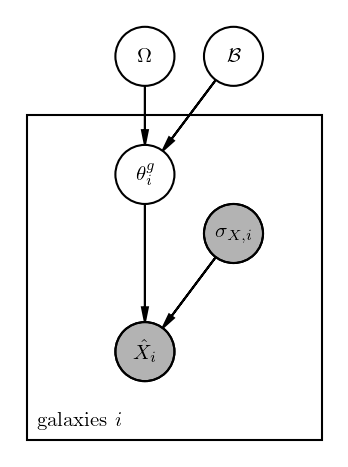
\includegraphics[width=0.4\textwidth]{figs/graph.png} 
    \caption{
    }\label{fig:graph}
\end{center}
\end{figure}



\begin{align}\label{eq:popinf}
p(\Omega, \mathcal{B} \given \{{\bfi X_i}\}) 
    =&~\frac{p(\Omega, \mathcal{B})~p(\{{\bfi X_i}\} \given \Omega, \mathcal{B})}{p(\{{\bfi X_i}\})}\\
    =&~\frac{p(\Omega, \mathcal{B})}{p(\{{\bfi X_i}\})}\int p(\{{\bfi X_i}\}
    \given \{\theta^g_i\})~p(\{\theta^g_i\} \given \Omega, \mathcal{B})~{\rm d}\{\theta^g_i\}.\\
    =&~\frac{p(\Omega, \mathcal{B})}{p(\{{\bfi X_i}\})}\prod\limits_{i=1}^N\int
    p({\bfi X_i} \given \theta^g_i)~p(\theta^g_i \given \Omega, \mathcal{B})~{\rm d}\theta^g_i\\
    =&~\frac{p(\Omega, \mathcal{B})}{p(\{{\bfi X_i}\})}\prod\limits_{i=1}^N\int
    \frac{p(\theta^g_i \given {\bfi X_i})~p({\bfi
    X_i})}{p(\theta^g_i)}~p(\theta^g_i \given \Omega, \mathcal{B})~{\rm d}\theta^g_i\\
    =&~p(\Omega, \mathcal{B})\prod\limits_{i=1}^N\int \frac{p(\theta^g_i \given
    {\bfi X_i})~p(\theta^g_i \given \Omega, \mathcal{B})}{p(\theta^g_i)}~{\rm d}\theta^g_i. 
\intertext{
    We estimate the integral using $S_i$ Monte Carlo samples from the
    individual posteriors $p(\theta^g_i \given {\bfi X_i})$: 
}
    \approx&~p(\Omega, \mathcal{B})\prod\limits_{i=1}^N\frac{1}{S_i}\sum\limits_{j=1}^{S_i}
    \frac{p(\theta^g_{i,j} \given \Omega, \mathcal{B})}{p(\theta^g_{i,j})}.
\end{align} 


% --- summary ---  
\input{summary}

\section*{Acknowledgements}
It's a pleasure to thank

\appendix

\bibliographystyle{mnras}
\bibliography{cgpop} 
\end{document}
